\begin{frame}{Mehrfachvererbung oder Interfaces?}{Was ist besser?}
\textbf{Was kann Mehrfachvererbung, das Interfaces nicht können?}
    \begin{itemize}[<+->]
        \item Kurzgesagt: Funktional lässt sich beides äquivalent nutzen
        \item Der Unterschied liegt vielmehr in formaler Betrachtung der OOP
        \item Mehrfachvererbung birgt aber viele Risiken
        \begin{itemize}
            \item Diamond-Problem
            \item Komplexe (=undurchsichtige) Vererbungshierarchien
            \item Falsche Verwendung
        \end{itemize}
    \end{itemize}
\end{frame}

\begin{frame}{Diamond-Problem}{Visuelle Darstellung}
    \begin{figure}
        \centering
        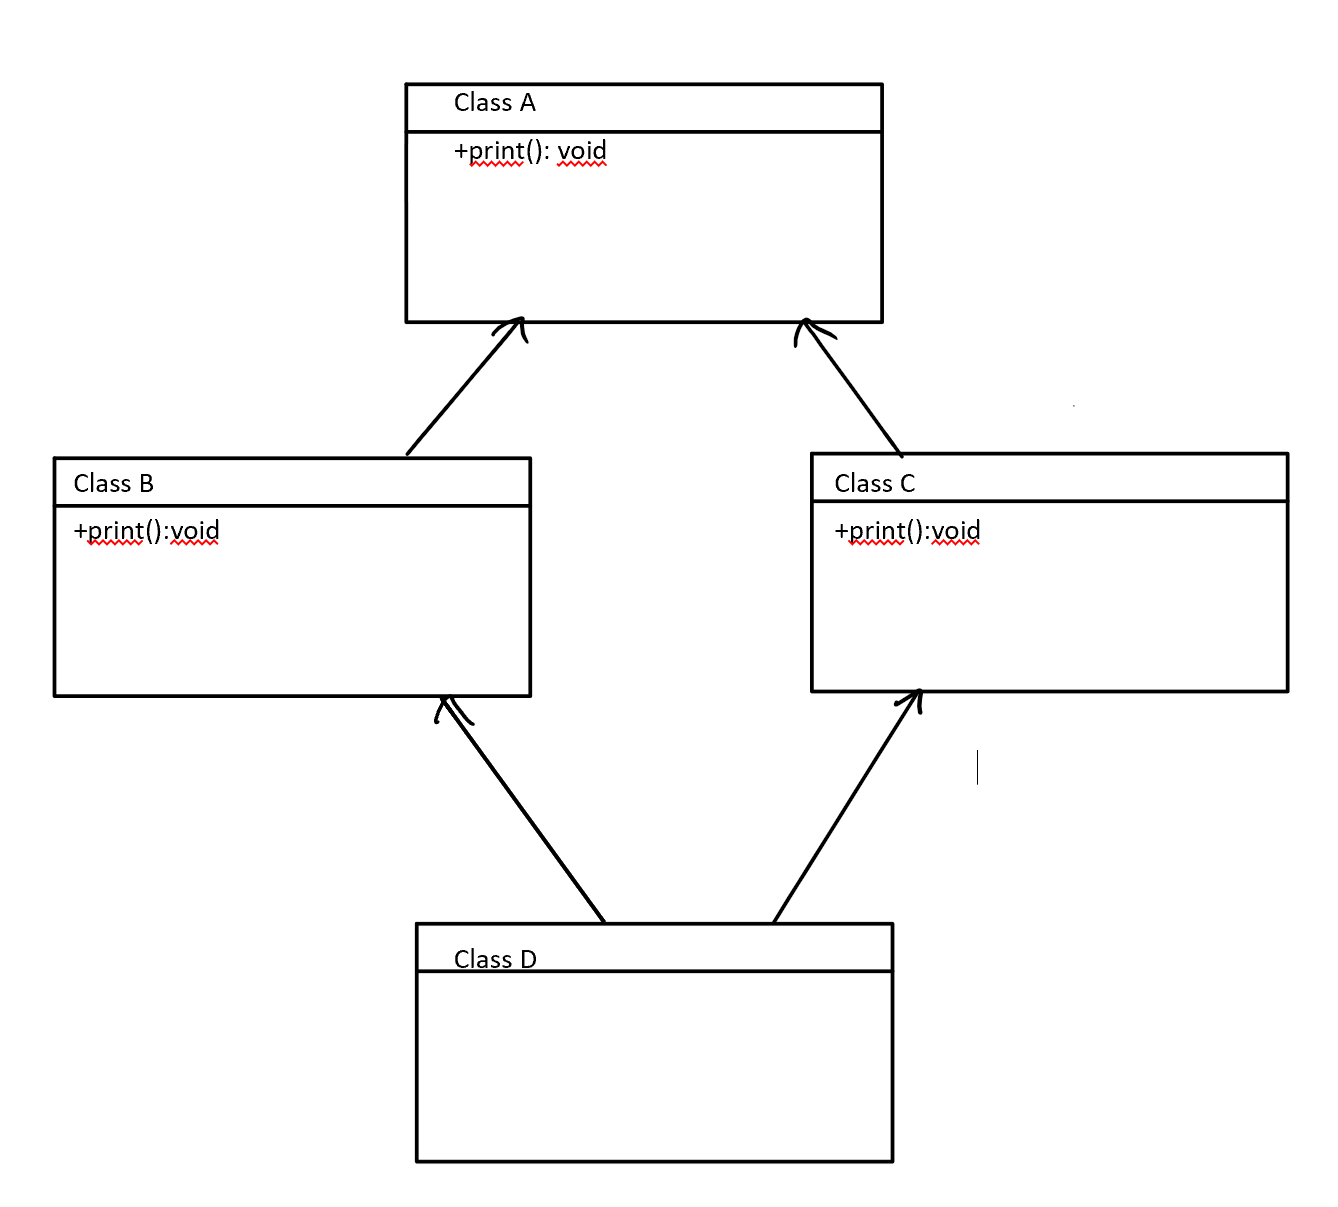
\includegraphics[height=4.5cm]{graph/diamond}
    \end{figure}
\end{frame}

\begin{frame}{Diamond-Problem}{Kurze Erklärung}
    \begin{itemize}
        \item Tritt auf, wenn die "`Großvaterklasse"' von zwei Basisklassen gleich ist
        \item Führt zu einer Mehrdeutigkeit in Methoden und Member Variablen
        \item Diese wird jedoch in den meisten Sprachen durch den Compiler abgefangen
        \item Diamond Problem \textit{kann} auch in Java auftreten
        \begin{itemize}
            \item Weil Default-Implementierungen von Interfaces erlaubt sind
            \item Werden auch durch Compiler erkannt
            \item Entwickler \textbf{muss} Klassenspezifische Implementierung erstellen
        \end{itemize}
    \end{itemize}
\end{frame}

\begin{frame}[fragile]{Diamond-Problem}{Am Java Beispiel}
\lstset{style=java}
\begin{lstlisting}
public interface A{
    public void say(){
        print("I am A!");
    }
}

public interface B{
    public void say(){
        print("I am B");
    }
}

public class C implements A,B{
    //Compilerfehler, weil say() mehrdeutig ist!
}
\end{lstlisting}
\end{frame}

\begin{frame}{Das Problem der Mehrfachvererbung}
    \begin{itemize}
        \item Oft falsch verwendet
        \item Besonders bei Anfängern
        \item Wo keine Mehrfachvererbung ist, kann sie nicht falsch verwendet werden $\Rightarrow$ Der Java Ansatz
        \item Statt Mehrfachvererbung hilft oft:
        \begin{itemize}
            \item Assoziation
            \item Aggregation
            \item Komposition
            \item Delegation
        \end{itemize}
    \end{itemize}
\end{frame}

\begin{frame}{Assoziation}
\begin{itemize}
    \item Beziehung zwischen zwei Objekten
    \item Es besteht jedoch keine Abhängigkeit
    \item Beide Objekte können unabhängig voneinander existieren
    \item Beispiel: Relation zwischen Sprecher und Zuhörer
\end{itemize}
\begin{figure}
    \centering
    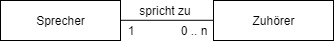
\includegraphics[width=0.8\textwidth]{graph/association}
\end{figure}
\end{frame}

\begin{frame}{Aggregation}
\begin{itemize}
    \item Sonderfall der Assoziation
    \item Hier eine unidirektionale Beziehung (\textbf{"`benötigt ein"'} Beziehung)
    \item Kindobjekt kann unabhängig von Elternobjekt existieren
    \item Aber Elternobjekt nicht ohne Kind
    \item Beispiel: Auto und Räder
    \begin{itemize}
        \item Räder können auch ohne Auto sinnvoll sein
        \item Autos ohne Räder eher weniger...
    \end{itemize}
\end{itemize}
\begin{figure}
    \centering
    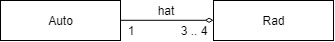
\includegraphics[width=0.8\textwidth]{graph/aggregation}
\end{figure}
\end{frame}

\begin{frame}{Komposition}
    \begin{itemize}
        \item Sonderfall der Aggregation
        \item Strenge Abhängigkeit zwischen kind- und Elternobjekt
        \item Beide können nicht unabhängig voneinander existieren
        \item Beispiel: Mensch und Herz
    \end{itemize}
\begin{figure}
    \centering
    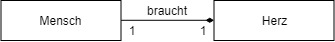
\includegraphics[width=0.8\textwidth]{graph/composition}
\end{figure}
\end{frame}

\begin{frame}{Delegation}
    \begin{itemize}
        \item Ist ein alternativer Ansatz zur Vererbungshierarchien
        \item Hierbei wird ein Objekt als Instanzvariable genutzt
        \item Funktionsaufrufe werden "`durchgereicht"' an dieses
        \item Vorteil gegenüber Vererbung/Interfaces:
        \begin{itemize}
            \item Nicht alle Methoden müssen nach außen sichtbar gemacht werden
            \item Für Delegate kann spezielle Unterklasse genutzt werden
        \end{itemize}
    \end{itemize}
\end{frame}

\begin{frame}[fragile]{Delegation}{Codebeispiel}
\lstset{style=java}
\begin{lstlisting}
public class Delegate(
    public void print(){
        System.out.println("I am a Delegate!");
    }    
    public void sayHello(){
        System.out.println("Hello!");
    }
)

public Class Example{
    private Delegate del = new Delegate();
    
    public void print(){
        del.print();
    }
}
\end{lstlisting}
\end{frame}

\begin{frame}{Schlechte Mehrfachvererbung}
    \begin{itemize}
        \item Wir haben eine Klasse \texttt{Rad} und \texttt{Motor}
        \item Man möchte nun eine \texttt{Auto} Klasse implementieren
        \item Ein unerfahrener Nutzer denkt:
        \begin{itemize}
            \item Ein Auto braucht Fähigkeiten vom \texttt{Rad}
            \item ...und vom \texttt{Motor}
            \item und entwirft folgende Klasse:
        \end{itemize}
    \end{itemize}
\end{frame}

\begin{frame}{Schlechte Mehrfachvererbung}{Am Beispiel}
    \begin{figure}
        \centering
        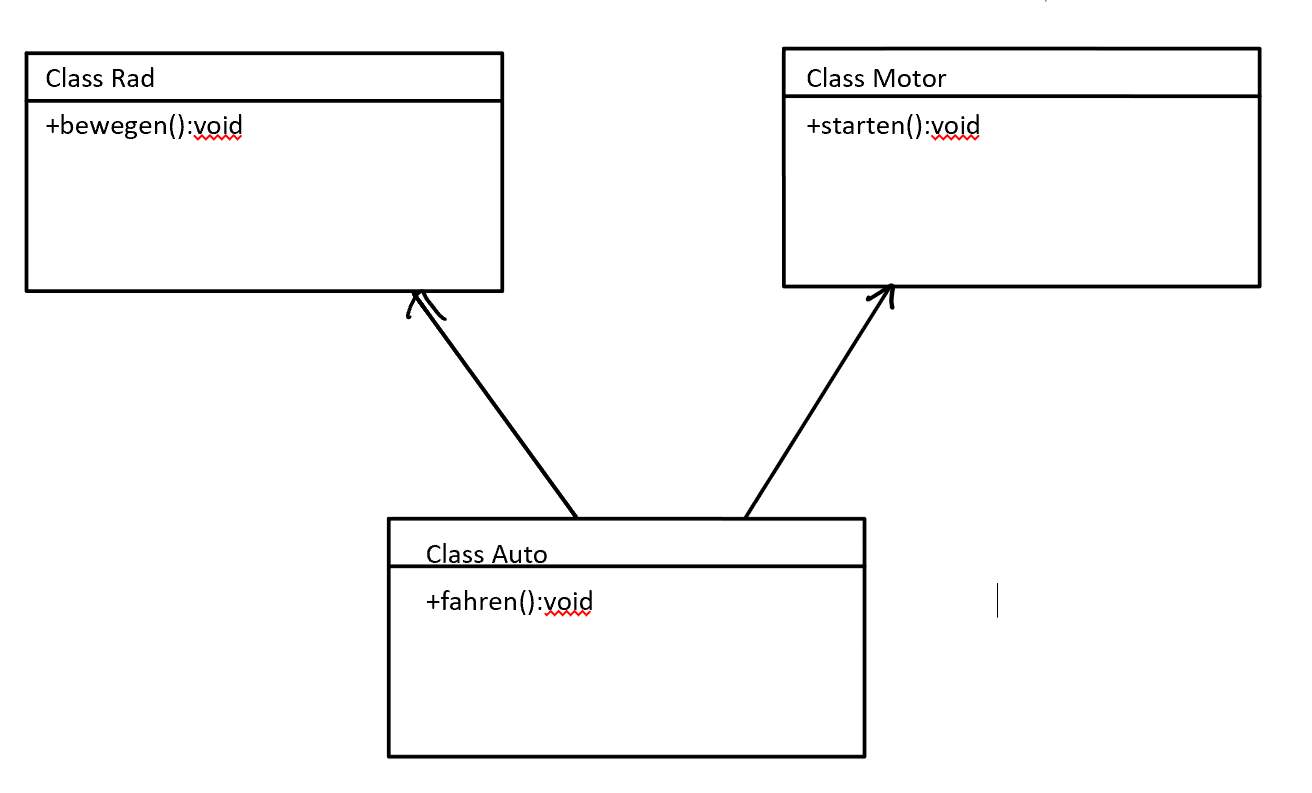
\includegraphics[height=4.5cm]{graph/badMI}
    \end{figure}
\end{frame}

\begin{frame}{Gute Verwendung von Mehrfachvererbung}
\begin{itemize}
    \item Sind relativ selten
    \item Wenige reale Anwendungsfälle
    \item Ein Beispiel: "`Mix-in Klassen"'
    \begin{itemize}
        \item Nutzt im Grunde Mehrfache Verkettung von Template Klassen (Generics)
        \item Link für mehr Info(C++): \href{http://www.thinkbottomup.com.au/site/blog/C\%20\%20_Mixins_-_Reuse_through_inheritance_is_good}{Mix-in} (Siehe \cite{mixin})
    \end{itemize}
\end{itemize}
\end{frame}

\begin{frame}{Der Zusammenhang zu Interfaces}
    \begin{itemize}[<+->]
        \item Laut formalen OOP:
        \begin{itemize}
            \item Definiert \textit{Vererbung} eine \textbf{"`ist ein"'} Beziehung
            \item Und ein \textit{Interface} eine \textbf{"`Hat die Fähigkeit"'} Beziehung
        \end{itemize}
        \item Heißt, formal "`darf"' man ein Interface nicht als Mehrfachvererbung betrachtet werden
        \item ...ist aber irgendwie nicht weit davon weg
        \item Verstößt Java damit gegen die Prinzipien der OOP?
        \begin{itemize}[<handout:0>]
            \item Ganz klares: "`Jain"'
            \item Kaum eine Sprache erfüllt alle Anforderungen an OOP
        \end{itemize}
    \end{itemize}
\end{frame}

\begin{frame}{"`Richtige"' Eigenschaften von Interfaces}
    \begin{itemize}
        \item Rein abstrakte Definition von Schnittstellen
        \item Keine Attribute
        \item Keine Assoziationen
        \item Definiert eine Menge von Operationen $\Rightarrow$ Eigentlich ohne Implementierung
    \end{itemize}
\end{frame}
